\chapter{Background} 
\label{chapter:background}
The traditional approach for finding relevant documents for a given query
is to count repetitions of query terms in the documents. Different weight
schemes for these counts lead to a variety of TF-IDF ranking features. How-
ever, the basic forms of such a ranking system only consider query terms,
under the assumption that non-query terms are less useful for document
ranking. This makes such ranking systems incapable of capturing the deep
semantic meaning of the text all by itself. One of the most popular 
approaches in the field of semantic similarity is word embedding models. And it can be further 
improved in different ways to obtain better results.

\section{Summary of relevant approaches}

Word embedding models have become the benchmark for semantic similarity extraction in the Natural language field, different kinds of word level embeddings such as {cite word2vec} ,{Glove} and {swivel} has-been presented. Another interesting form of
embeddings is a recent work by Google named Swivel [Shazeer et al., 2016].

Some commendable efforts have been made to go beyond word level representations  \cite{mitchell2010composition}  \cite{zanzotto2010estimating} 
\cite{yessenalina2011compositional}  \cite{grefenstette2013multi}  \cite{mikolov2013distributed}. A simple approach is to use the weighted average of all the words in the document. But weighted averaging of word vectors loses the word order. A more sophisticated approach is combining the word vectors
in an order given by a parse tree of a sentence, using
matrix-vector operations \cite{socher2011dynamic}. A drawback of such an approach is that it only works on sentences as it relies on parse trees.

An extension to Word2Vec known as Doc2Vec was proposed in \cite{le2014distributed} to work on input sequences of
variable length.

 \cite{bojanowski2016enriching} propose another extention of word2v model by learning word
 representations while taking into account morphology.
 They model morphology by considering subword
 units, and representing words by a sum of its character
 n-grams

\cite{ghosh2016characterizing} introduce a vocabulary driven Word2Vec method known as Dis2Vec which is
used to generate disease-specific word embeddings from unstructured health-
related news corpus. The input corpus D consists of a collection of word context pairs.The input corpus $D$ consists of a collection of word context pairs. Based on the vocabulary $ V$, we can categorize the word context pairs into three types as shown
below:
\\
\begin{itemize}
	\item $ D(d) = {(w, c): w \in V ∧c \in V }$, i.e. both the word w and the context c are in V
	\item $D(\rightharpoondown d) = {(w, c): w \notin V ∧c \notin V }$, i.e. neither the word w nor the context c are in V
	\item $D(\rightharpoondown d) = {(w, c): w \in V \oplus c \in V }$, i.e. either the word w is in V or the context c is in V but both cannot be in V
\end{itemize}

All the above mentioned word embedding models learn word embeddings from co-occurrence information in corpora.
One drawback of learning word embeddings by by this approach is that such methods will generally fail to tell synonyms from
antonyms (Mohammad et al., 2008). For example, words like east and west
or expensive and cheaper appear in near-identical contexts, which means
that distributional models produce very similar word vectors for such words.
\cite{mrksic:2016:naacl} proposed a novel counter-fitting method which injects antonymy and
synonymy constraints into vector space representations in order to circumvent this issue.

An alternative to
the bag-of-words approach is to derive contexts
based on the syntactic relations the word participates
in as proposed by {dependency-based-word-embeddings}. 


\subsection{Word Embeddings} 
Word embedding is a way of transforming human readable words to the real number vector 
space of the desired dimension. The transformation can, for example, be learned by a very simple neural network, that tries to predict words from its context \cite{NIPS2013_5021}. Embeddings 
can be learned from any sufficiently large volume of text data. There are propositions that embeddings  
as vectors containing latent features of words will differ if the corpora they are trained on are different \cite{bollegala2015unsupervised}. So for 
tasks in the medical domain it is better to use embeddings trained on medical texts. There are also other ways of obtaining embeddings besides neural networks, such 
as learning statistical information about occurrences of words in texts or mixed models incorporating the best of other methods. Three types of word embeddings were considered 
for experiments in this work.

\paragraph{Word2Vec} Word2Vec model uses distributed vector representation of words, a well-known framework for learning word vectors as shown in the Figure \ref{fig:Word2Vec model}. The task is to learn to predict a word given other words in the context.
More formally, given a sequence of training words
$w_{1}, w_{2}, w_{3}, ..., w_{T} $, the objective of the word vector model is to maximize the average log probability
\\
\begin{equation}
\frac{1}{T} \sum_{t=K}^{T-K} \log p(w_{t} \mid w_{t-1},....,w_{t+1}) 
\end{equation}

	\begin{figure}[h]
		\centering
		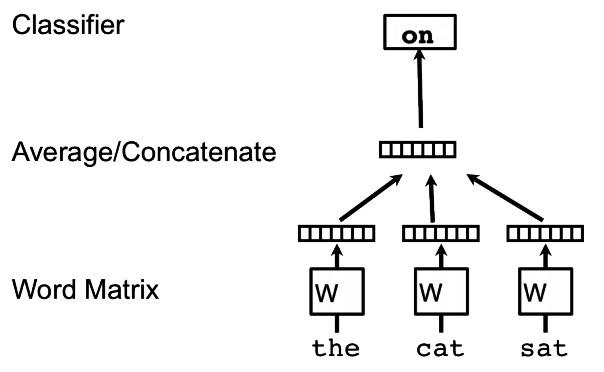
\includegraphics[width=8cm, height=5cm]{w2v.png}
		\caption{A framework for learning word vectors. Context of
			three words (“the,” “cat,” and “sat”) is used to predict the fourth
			word (“on”). The input words are mapped to columns of the matrix
			W to predict the output word.}
		\label{fig:Word2Vec model}
	\end{figure}
\paragraph{GloVe} GloVe was introduced in \cite{pennington2014glove} as a result of trying 
to make vector space representations of words more interpretable. It connects two ideas of 
embedding - usage of matrix factorisation and local context windows. Thus, it uses whole 
corpus words co-occurrences but also takes into account local context. The evaluation showed that 
this model outperforms other embeddings models of that time on the tasks of word analogy, 
Named Entity Recognition.

\paragraph{Swivel} Swivel is one of the latest models for obtaining word embeddings 
\cite{DBLP:journals/corr/ShazeerDEW16}. The idea behind this method is to factorise the whole 
matrix of co-occurrences constructed from the text corpora by dividing it into smaller parts and 
parallelising computations. The idea is taken both from GloVe model and skip-gram model 
(Word2Vec).

\paragraph{Doc2Vec}Doc2Vec is capable of constructing representations of input sequences of
variable length. Unlike some of the previous approaches, it is general and
applicable to texts of any length: sentences, paragraphs, and documents. In
Doc2Vec framework (see Figure \ref{fig:doc2vec model}), every document is mapped to a unique
vector, and every word is also mapped to a unique vector. The document
vector and word vectors are averaged or concatenated to predict the next
word in a context. The only difference to a Word2Vec model is the additional
document token.It acts as a memory that remembers what is missing from
the current context or the topic of the document. The document vectors and
word vectors are trained using stochastic gradient descent and the gradient
is obtained via back-propagation.

	\begin{figure}[h]
		\centering
		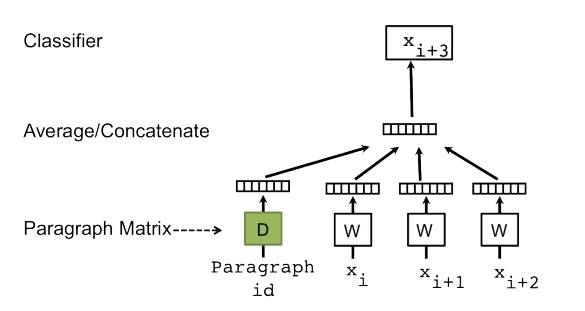
\includegraphics[width=8cm, height=5cm]{para}
		\caption[]{A framework for learning paragraph vector. This framework
			is similar to the framework presented in Figure 1; the only
			change is the additional paragraph token that is mapped to a vector
			via matrix D. In this model, the concatenation or average of
			this vector with a context of three words is used to predict the
			fourth word. The paragraph vector represents the missing information
			from the current context and can act as a memory of the
			topic of the paragraph.}
		\label{fig:doc2vec model}
	\end{figure}
	